\chapter{Quantum Mechanics and the Harmonic Oscillator: Ladder Operators}
\label{chap:e04}

\begin{chapteropening}
So far we have kept saying ``photon'' without ever seriously asking: where does a photon actually come from? It is not a little ball hidden in the vacuum ahead of time; it is a single ``step up'' of some vibrating mode. To make this statement precise, we must first return to the simplest and most important system in all of quantum mechanics: the harmonic oscillator.

This chapter has a single central question: for a system that vibrates back and forth, why can its energy take only discrete, evenly spaced values? The answer hides in two operators: one that moves you ``down one rung,'' one that moves you ``up one rung.'' They are called ladder operators. Starting from the ordinary position and momentum, we will build these two operators without skipping a single step, prove that they satisfy an exceptionally clean commutation relation, and then use them to read off the energy spectrum, the number states, and the zero-point energy all at once. This is the first cornerstone of the whole book's answer to ``where do photons come from'': once you have digested the algebra of this chapter, every later discussion of coherent states, thermal states, and photon statistics will be nothing but a generalization of it.
\end{chapteropening}

\section{A Minimal Review of Quantum Mechanics}
\label{sec:e04-review}

Before we get our hands dirty, let us lay out on the table a few quantum-mechanical ``tools'' that we will use over and over. This section proves nothing; it merely relights things you have most likely seen once before. If every item feels familiar, that is precisely the sign that you are ready.

\paragraph{State vectors.}
The state of a quantum system at a given moment is represented by a vector \(|\psi\rangle\), read ``ket psi.'' You may picture it as an arrow living in an abstract space (a Hilbert space). Its dual partner is written \(\langle\psi|\) (``bra psi''), and joining the two, \(\langle\psi|\psi\rangle\), gives the squared length of that arrow. Physically we always require a state to be normalized:
\[
  \langle\psi|\psi\rangle=1,
\]
because the total probability that ``the system is in some state'' must be 1.

\paragraph{Operators and eigenvalues.}
To every physical measurement one can make on the system (energy, position, momentum, \ldots) there corresponds an operator, which we denote with a hatted letter, for example \(\hat H,\hat x,\hat p\). An operator acting on a state produces a new state. In particular, if a state satisfies
\[
  \hat A\,|a\rangle = a\,|a\rangle,
\]
we say \(|a\rangle\) is an eigenstate of \(\hat A\), and the number \(a\) is the corresponding eigenvalue. Physically, only when the system is exactly in \(|a\rangle\) will a measurement of \(A\) yield \(a\) with certainty. Operators corresponding to observables are all Hermitian (\(\hat A^\dagger=\hat A\)), which guarantees real eigenvalues: the numbers we read out must of course be real.

\paragraph{Expectation values.}
If the state is not an eigenstate, the measurement outcome fluctuates and we can only speak of an average. Measuring \(A\) on the state \(|\psi\rangle\), the average over many repetitions is the expectation value
\begin{equation}
  \langle A\rangle \equiv \langle\psi|\,\hat A\,|\psi\rangle .
  \label{eq:e04-expectation}
\end{equation}
\begin{formulaexplain}
\(\langle A\rangle\) is the mean measured value of the observable \(A\) on the state \(|\psi\rangle\). Simply sandwich the operator \(\hat A\) between \(\langle\psi|\) and \(|\psi\rangle\). If the state is normalized, this is the average in the genuine sense.
\end{formulaexplain}
Here \(\hat A\) is the operator corresponding to the quantity to be measured, and \(|\psi\rangle\) is the current (normalized) state of the system. Equation \eqref{eq:e04-expectation} is the single ``value-extraction'' device we will use again and again in this chapter: once the state and the operator are known, any average is computed from it. It has no unit ambiguity: the units are fixed entirely by \(\hat A\), for example when \(\hat A=\hat H\), \(\langle H\rangle\) is an energy (erg).

\paragraph{Commutators.}
The order in which two operators act generally cannot be swapped, and this ``non-commutativity'' is precisely the fundamental divide between quantum and classical mechanics. We measure it with the commutator:
\begin{equation}
  [\hat A,\hat B]\equiv \hat A\hat B-\hat B\hat A .
  \label{eq:e04-commutator}
\end{equation}
\begin{formulaexplain}
\([\hat A,\hat B]\) measures the difference between ``\(B\) then \(A\)'' and ``\(A\) then \(B\).'' If it vanishes, the two quantities can be measured precisely at the same time; if it does not, they ``fight'' each other.
\end{formulaexplain}
\(\hat A\hat B\) means letting \(\hat B\) act first and then \(\hat A\) (operators act on states from right to left). If \([\hat A,\hat B]=0\), we say the two operators commute; they share common eigenstates and can have definite values simultaneously. If not, they cannot. When we later build the ladder operators, nearly every simplification step amounts to repeatedly shuffling this \(\hat A\hat B-\hat B\hat A\). One identity we will need shortly (verified by direct expansion) is
\[
  [\hat A,\hat B\hat C]=[\hat A,\hat B]\hat C+\hat B[\hat A,\hat C].
\]

\paragraph{The canonical commutation relation.}
Of all commutators, the most basic is the canonical commutation relation between position and momentum:
\begin{equation}
  [\hat x,\hat p]=i\hbar .
  \label{eq:e04-xp}
\end{equation}
\begin{formulaexplain}
\(\hat x\) is the position operator, \(\hat p\) the momentum operator, and \(\hbar\) the reduced Planck constant. They do not commute; they differ by a pure imaginary constant \(i\hbar\). This is the ``foundation brick'' of all of quantum mechanics.
\end{formulaexplain}
In \eqref{eq:e04-xp}, \(\hat x\) has the dimension of length (cm) and \(\hat p\) the dimension of momentum (\(\mathrm{g\,cm\,s^{-1}}\)); their product has the dimension of action (\(\mathrm{erg\,s}\)), consistent with \(\hbar\) (\(\hbar\simeq1.05\times10^{-27}\,\mathrm{erg\,s}\)). Note that the right-hand side is a pure number times the identity operator, independent of the state; this is exactly why it is ``fundamental.'' All the algebra in the rest of this chapter, at bottom, uses only this one relation \([\hat x,\hat p]=i\hbar\); everything else is logical deduction.

\paragraph{The uncertainty relation.}
Two non-commuting quantities cannot be determined with unlimited precision at the same time; this is the uncertainty relation. Its general form is the Robertson inequality: for any two Hermitian operators \(\hat A,\hat B\), their standard deviations in any state satisfy
\[
  \Delta A\,\Delta B\ \ge\ \frac12\big|\langle[\hat A,\hat B]\rangle\big| .
\]
The right-hand side of this inequality is set precisely by the commutator: the more two quantities ``fail to commute,'' the less they can be determined together. We will not prove it in this review; we simply take it as a known result and use it. Now set \(\hat A=\hat x,\hat B=\hat p\) and substitute the canonical commutation relation \eqref{eq:e04-xp}, \([\hat x,\hat p]=i\hbar\); the right-hand expectation value \(\langle i\hbar\rangle=i\hbar\) (a pure constant, independent of state), so \(\tfrac12|\langle[\hat x,\hat p]\rangle|=\tfrac12|i\hbar|=\hbar/2\), giving the most famous instance:
\[
  \Delta x\,\Delta p\ \ge\ \frac{\hbar}{2},
\]
where \(\Delta x=\sqrt{\langle \hat x^2\rangle-\langle\hat x\rangle^2}\) is the standard deviation of position and \(\Delta p\) is defined analogously. It tells us that a quantum state cannot simultaneously push both position and momentum down to zero fluctuation. Remember this ``minimum area \(\hbar/2\),'' because the ground state of the harmonic oscillator is exactly the state that saturates this inequality; it is the ``quietest'' vibration that quantum fluctuations allow. That ends this section; our toolkit is now complete.

\section{The Quantum Harmonic Oscillator and the Construction of Ladder Operators}
\label{sec:e04-ladder}

Now to the main event. Picture a small ball tied to a spring vibrating back and forth, or two atoms in a diatomic molecule stretching relative to each other, or (and this is what we really care about) the oscillation of a single mode of the electromagnetic field. Mathematically they are the same system: the harmonic oscillator. In quantum mechanics, its Hamiltonian (the energy operator) is
\begin{equation}
  \hat H=\frac{\hat p^2}{2m}+\frac{1}{2}m\omega^2\hat x^2 .
  \label{eq:e04-hamiltonian}
\end{equation}
\begin{formulaexplain}
The first term \(\hat p^2/2m\) is the kinetic energy, the second \(\tfrac12 m\omega^2\hat x^2\) is the spring potential energy. \(m\) is the mass and \(\omega\) the angular frequency of vibration. The whole expression is the quantum version of ``kinetic plus potential energy.''
\end{formulaexplain}
In \eqref{eq:e04-hamiltonian}, \(m\) is the mass (g), \(\omega\) the angular frequency (\(\mathrm{rad\,s^{-1}}\)), and \(\hat x,\hat p\) the position and momentum operators of the previous section. The whole thing has the dimension of energy (erg). Classically, this system oscillates sinusoidally at frequency \(\omega\), and its energy can take any positive value continuously. The quantum question is: what do the eigenvalues of \(\hat H\) (that is, the allowed energies) look like?

Solving the differential equation directly is of course possible, but it would drown us in special functions. There is a far more elegant path: factor \(\hat H\). Notice that \(\hat p^2/2m+\tfrac12 m\omega^2\hat x^2\) has the shape of \(a^2+b^2\), and \(a^2+b^2=(a-ib)(a+ib)\), except that \(\hat x\) and \(\hat p\) do not commute, so the factorization leaves behind a ``tail,'' and that tail hides all the physics. To this end we define two new operators:
\begin{equation}
  \hat a=\sqrt{\frac{m\omega}{2\hbar}}\left(\hat x+\frac{i\,\hat p}{m\omega}\right),
  \qquad
  \hat a^\dagger=\sqrt{\frac{m\omega}{2\hbar}}\left(\hat x-\frac{i\,\hat p}{m\omega}\right).
  \label{eq:e04-adef}
\end{equation}
\begin{formulaexplain}
\(\hat a\) is the annihilation operator, \(\hat a^\dagger\) the creation operator; the two are Hermitian conjugates of each other. They package the dimensionful \(\hat x,\hat p\) into a dimensionless combination and are the ``keys'' to the energy ladder.
\end{formulaexplain}
First a word on dimensions, to confirm these two definitions are ``clean.'' The coefficient \(\sqrt{m\omega/2\hbar}\) has dimension \(\sqrt{\mathrm{g}\cdot\mathrm{s^{-1}}/\mathrm{erg\,s}}=\mathrm{cm^{-1}}\) (since \(\mathrm{erg}=\mathrm{g\,cm^2\,s^{-2}}\)); multiplied by \(\hat x\) of dimension cm, it gives a pure number. Likewise \(\hat p/(m\omega)\) has dimension \(\mathrm{g\,cm\,s^{-1}}/(\mathrm{g\,s^{-1}})=\mathrm{cm}\), which also becomes a pure number. So \(\hat a,\hat a^\dagger\) are both dimensionless operators; this matters, because they count ``which rung'' and should not carry units to begin with. Since \(\hat x,\hat p\) are Hermitian, taking the Hermitian conjugate of \eqref{eq:e04-adef} (\(i\to -i\)) immediately shows that \(\hat a\) and \(\hat a^\dagger\) are indeed conjugates.

\paragraph{Solving back for \(\hat x,\hat p\).}
After defining these, we will often need to invert and express \(\hat x,\hat p\) through \(\hat a,\hat a^\dagger\). Just add and subtract the two lines of \eqref{eq:e04-adef}: adding cancels the imaginary parts, subtracting cancels the real parts,
\[
  \hat a+\hat a^\dagger=\sqrt{\frac{m\omega}{2\hbar}}\,(2\hat x),
  \qquad
  \hat a-\hat a^\dagger=\sqrt{\frac{m\omega}{2\hbar}}\,\frac{2i\,\hat p}{m\omega}.
\]
Hence
\begin{equation}
  \hat x=\sqrt{\frac{\hbar}{2m\omega}}\,(\hat a+\hat a^\dagger),
  \qquad
  \hat p=-i\sqrt{\frac{m\omega\hbar}{2}}\,(\hat a-\hat a^\dagger).
  \label{eq:e04-xp-in-a}
\end{equation}
\begin{formulaexplain}
Position and momentum rewritten as combinations of the creation and annihilation operators. \(\hat x\) corresponds to the ``symmetric'' combination \(\hat a+\hat a^\dagger\), \(\hat p\) to the ``antisymmetric'' combination \(\hat a-\hat a^\dagger\), each with a dimensionful prefactor.
\end{formulaexplain}
These two relations will be used repeatedly later: any quantity containing \(\hat x,\hat p\) (for instance the electric field, which is proportional to \(\hat x\)) can be translated into the language of creation and annihilation operators. The prefactor \(\sqrt{\hbar/2m\omega}\) has exactly the dimension cm, and \(\sqrt{m\omega\hbar/2}\) exactly the units of momentum, dimensionally self-consistent.

\paragraph{The key step: computing \([\hat a,\hat a^\dagger]\).}
This is the single most important piece of algebra in the chapter, and we do it without skipping a step. Substitute the definitions \eqref{eq:e04-adef} into the commutator, first pulling out the constant coefficient \(m\omega/2\hbar\):
\[
  [\hat a,\hat a^\dagger]
  =\frac{m\omega}{2\hbar}
  \left[\hat x+\frac{i\hat p}{m\omega},\ \hat x-\frac{i\hat p}{m\omega}\right].
\]
The commutator is linear in both slots, so expand it into four terms:
\[
  \left[\hat x+\tfrac{i\hat p}{m\omega},\ \hat x-\tfrac{i\hat p}{m\omega}\right]
  =[\hat x,\hat x]
  -\frac{i}{m\omega}[\hat x,\hat p]
  +\frac{i}{m\omega}[\hat p,\hat x]
  -\frac{i^2}{(m\omega)^2}[\hat p,\hat p].
\]
Now handle each term. Any operator commutes with itself, so \([\hat x,\hat x]=[\hat p,\hat p]=0\), and the first and fourth terms vanish outright. The middle two use the canonical commutation relation \eqref{eq:e04-xp}: \([\hat x,\hat p]=i\hbar\), and \([\hat p,\hat x]=-[\hat x,\hat p]=-i\hbar\). Substituting:
\[
  =-\frac{i}{m\omega}(i\hbar)+\frac{i}{m\omega}(-i\hbar)
  =-\frac{i^2\hbar}{m\omega}-\frac{i^2\hbar}{m\omega}
  =\frac{\hbar}{m\omega}+\frac{\hbar}{m\omega}
  =\frac{2\hbar}{m\omega},
\]
where we used \(i^2=-1\). Multiplying back by the leading coefficient:
\[
  [\hat a,\hat a^\dagger]=\frac{m\omega}{2\hbar}\cdot\frac{2\hbar}{m\omega}=1.
\]
And so we obtain the ``main theorem'' of the chapter:
\begin{equation}
  [\hat a,\hat a^\dagger]=1 .
  \label{eq:e04-aacomm}
\end{equation}
\begin{formulaexplain}
The commutator of the creation and annihilation operators equals 1. This extraordinarily simple relation is the source of the entire quantum structure of the harmonic oscillator (and of every field mode to come); the energy levels, the photons, and the zero-point energy all grow out of it.
\end{formulaexplain}
Savor how clean this equation is: the dimensionful \(\hat x,\hat p\), the dimensionful \(m,\omega,\hbar\), all cancel, leaving nothing but a bare 1. It is dimensionless and independent of which particular oscillator we have. Equation \eqref{eq:e04-aacomm} will become the only commutation relation we need to remember; from this moment on we can almost forget \(\hat x,\hat p\) and work entirely within the algebra of \(\hat a,\hat a^\dagger\). By contrast, the creation operators among themselves and the annihilation operators among themselves of course commute: \([\hat a,\hat a]=[\hat a^\dagger,\hat a^\dagger]=0\).

\section{Rewriting the Hamiltonian with the Number Operator}
\label{sec:e04-numberH}

We built \(\hat a,\hat a^\dagger\) in order to simplify \(\hat H\). Now we translate \eqref{eq:e04-hamiltonian} into the language of creation and annihilation operators. The most economical approach is to first compute the combination \(\hat a^\dagger\hat a\) and see how far it is from \(\hat H\). Using the definitions \eqref{eq:e04-adef} and pulling out the coefficient:
\[
  \hat a^\dagger\hat a
  =\frac{m\omega}{2\hbar}
  \left(\hat x-\frac{i\hat p}{m\omega}\right)\!\left(\hat x+\frac{i\hat p}{m\omega}\right).
\]
Carefully multiply out the brackets (keeping the operator order, since they do not commute):
\[
  \left(\hat x-\tfrac{i\hat p}{m\omega}\right)\!\left(\hat x+\tfrac{i\hat p}{m\omega}\right)
  =\hat x^2+\frac{i}{m\omega}\hat x\hat p-\frac{i}{m\omega}\hat p\hat x-\frac{i^2}{(m\omega)^2}\hat p^2 .
\]
Combine the middle two terms; they form exactly a commutator: \(\dfrac{i}{m\omega}(\hat x\hat p-\hat p\hat x)=\dfrac{i}{m\omega}[\hat x,\hat p]=\dfrac{i}{m\omega}(i\hbar)=-\dfrac{\hbar}{m\omega}\). And the last term \(-i^2\hat p^2/(m\omega)^2=+\hat p^2/(m\omega)^2\). Hence
\[
  \hat a^\dagger\hat a
  =\frac{m\omega}{2\hbar}
  \left(\hat x^2+\frac{\hat p^2}{(m\omega)^2}-\frac{\hbar}{m\omega}\right)
  =\frac{m\omega}{2\hbar}\hat x^2+\frac{1}{2\hbar m\omega}\hat p^2-\frac12 .
\]
Multiply each of the first two terms by \(\hbar\omega\) to check whether they are \(\hat H\):
\[
  \hbar\omega\left(\frac{m\omega}{2\hbar}\hat x^2\right)=\frac12 m\omega^2\hat x^2,
  \qquad
  \hbar\omega\left(\frac{1}{2\hbar m\omega}\hat p^2\right)=\frac{\hat p^2}{2m}.
\]
These are exactly the potential and kinetic terms of \eqref{eq:e04-hamiltonian}! So \(\hbar\omega\,\hat a^\dagger\hat a=\hat H-\tfrac12\hbar\omega\), and rearranging gives
\begin{equation}
  \hat H=\hbar\omega\left(\hat a^\dagger\hat a+\frac12\right)
        =\hbar\omega\left(\hat n+\frac12\right),
  \qquad \hat n\equiv\hat a^\dagger\hat a .
  \label{eq:e04-Hn}
\end{equation}
\begin{formulaexplain}
The Hamiltonian is written as a simple linear function of the number operator \(\hat n=\hat a^\dagger\hat a\). The energy equals ``the number of excitation rungs \(\hat n\) plus half a rung'' times \(\hbar\omega\). That half rung is the zero-point energy.
\end{formulaexplain}
Here \(\hat n=\hat a^\dagger\hat a\) is called the number operator. It is Hermitian (\((\hat a^\dagger\hat a)^\dagger=\hat a^\dagger\hat a\)) and thus has real eigenvalues; we will see shortly that its eigenvalues are exactly \(0,1,2,\ldots\), that is, ``how many quanta are in this mode.'' Equation \eqref{eq:e04-Hn} completely simplifies the problem of finding the spectrum: once we know the eigenvalues of \(\hat n\), the energy is read off. Dimensionally, \(\hat n\) is dimensionless and \(\hbar\omega\) is an energy, all consistent.

\paragraph{Zero-point energy.}
The \(+\tfrac12\) in \eqref{eq:e04-Hn} is not a dispensable constant. Even when \(\hat n\) takes its minimum value 0, the energy is not zero but
\[
  E_0=\frac12\hbar\omega .
\]
This is the zero-point energy. Physically it is a direct consequence of the uncertainty relation: if the oscillator truly sat still at the bottom of the potential well, it would have both a definite position (\(x=0\)) and a definite momentum (\(p=0\)), violating \(\Delta x\,\Delta p\ge\hbar/2\). Quantum mechanics does not permit this ``absolute quiet,'' so even in the ground state the oscillator must retain a minimal amount of jitter, corresponding to the energy \(\tfrac12\hbar\omega\). This jitter is not a shortcoming of our measuring ability but a property of the vacuum itself; when we later discuss the light field, it is precisely this ``vacuum fluctuation'' that gives the physical starting point for shot noise and squeezed states. For an order of magnitude: for a visible-light mode with \(\nu\sim6\times10^{14}\,\mathrm{Hz}\), \(\hbar\omega=h\nu\simeq(6.6\times10^{-27})(6\times10^{14})\,\mathrm{erg}\simeq4\times10^{-12}\,\mathrm{erg}\approx2.5\,\mathrm{eV}\), so the zero-point energy is about 1.2 eV, by no means negligible.

\section{Number States: Energy, One Rung at a Time}
\label{sec:e04-numberstates}

Now let us read off the spectrum. By \eqref{eq:e04-Hn}, \(\hat H\) and \(\hat n\) differ only by a constant and a positive factor, so they share eigenstates. Let the eigenstate of \(\hat n\) be \(|n\rangle\) with eigenvalue \(n\):
\[
  \hat n\,|n\rangle=n\,|n\rangle .
\]
We call \(|n\rangle\) a number state, or Fock state. For now \(n\) is only an undetermined real number; the task of this section is to use the commutation relation \eqref{eq:e04-aacomm} to force it to be a non-negative integer, and along the way to find out exactly what \(\hat a,\hat a^\dagger\) give when acting on \(|n\rangle\).

\paragraph{Why the ladder operators ``climb the stairs.''}
First compute two key commutators. Using \([\hat a,\hat a^\dagger]=1\):
\[
  [\hat n,\hat a]=[\hat a^\dagger\hat a,\hat a]
  =\hat a^\dagger[\hat a,\hat a]+[\hat a^\dagger,\hat a]\hat a
  =0+(-1)\hat a=-\hat a,
\]
where we used the expansion identity \([\hat A\hat B,\hat C]=\hat A[\hat B,\hat C]+[\hat A,\hat C]\hat B\) and \([\hat a^\dagger,\hat a]=-1\). Likewise
\[
  [\hat n,\hat a^\dagger]=\hat a^\dagger[\hat a,\hat a^\dagger]+[\hat a^\dagger,\hat a^\dagger]\hat a
  =\hat a^\dagger(1)+0=+\hat a^\dagger .
\]
These two, \([\hat n,\hat a]=-\hat a\) and \([\hat n,\hat a^\dagger]=+\hat a^\dagger\), are the mechanical principle of the ``ladder.'' See how they work: let \(\hat n\) act on the new state \(\hat a|n\rangle\),
\[
  \hat n\,(\hat a|n\rangle)
  =(\hat a\hat n+[\hat n,\hat a])|n\rangle
  =(\hat a\hat n-\hat a)|n\rangle
  =\hat a(\hat n-1)|n\rangle
  =(n-1)\,\hat a|n\rangle .
\]
Read this line: \(\hat a|n\rangle\) is again an eigenstate of \(\hat n\), with the eigenvalue lowered by 1 to \(n-1\). So \(\hat a\) takes the system ``down one rung''; this is why it is called the annihilation operator. Entirely symmetrically,
\[
  \hat n\,(\hat a^\dagger|n\rangle)=(n+1)\,\hat a^\dagger|n\rangle,
\]
so \(\hat a^\dagger\) lifts the system ``up one rung'' and is the creation operator. This is the origin of the word ``ladder.''

\paragraph{The ladder must have a floor: \(n\) is a non-negative integer.}
Why can the steps not extend downward without bound into negative numbers? Because the eigenvalues of \(\hat n\) cannot be negative. Using \eqref{eq:e04-expectation}, compute the expectation of \(\hat n\) on the normalized \(|n\rangle\):
\[
  n=\langle n|\hat n|n\rangle=\langle n|\hat a^\dagger\hat a|n\rangle
  =\big(\hat a|n\rangle\big)^\dagger\big(\hat a|n\rangle\big)
  =\big\|\,\hat a|n\rangle\,\big\|^2\ \ge 0 .
\]
The crucial step is the middle one: \(\langle n|\hat a^\dagger\hat a|n\rangle\) is the inner product of the state \(\hat a|n\rangle\) with itself, that is, its squared length, and the squared length of any vector is non-negative. So \(n\ge0\). But \(\hat a\) lowers the eigenvalue by 1 each time it acts; if we started from some non-integer \(n\) and applied \(\hat a\) repeatedly, sooner or later we would drop below 0 and obtain a negative eigenvalue, a contradiction. The only way out is that this descending chain must land exactly on 0 at some step and stop there; that is, there exists a ground state \(|0\rangle\) satisfying
\begin{equation}
  \hat a\,|0\rangle=0 .
  \label{eq:e04-ground}
\end{equation}
\begin{formulaexplain}
The annihilation operator acting on the ground state gives zero (not the state \(|0\rangle\), but the zero vector). This says ``we have already reached the very bottom; there is no step further down.'' The ground state is the floor of the entire energy ladder.
\end{formulaexplain}
Only when the descending sequence is cut off at \(n=0\) by \eqref{eq:e04-ground} can negative eigenvalues be avoided. Working backward from this: climbing up from \(|0\rangle\) one step at a time with \(\hat a^\dagger\), the eigenvalues obtained can only be \(0,1,2,3,\ldots\). In other words, the excitation number of the harmonic oscillator can only be a non-negative integer, and this is precisely the mathematical root of ``photons can only come one at a time.''

\paragraph{Normalization factors: where the two \(\sqrt{\ }\) come from.}
We know \(\hat a|n\rangle\) is proportional to \(|n-1\rangle\), but what is the proportionality constant? This step must be worked out fully, because the factors in the later photon statistics all rely on it. Let \(\hat a|n\rangle=c_n|n-1\rangle\), where \(c_n\) is an undetermined constant and \(|n-1\rangle\) is already normalized. Take the squared norm of both sides:
\[
  \big\|\hat a|n\rangle\big\|^2
  =|c_n|^2\,\langle n-1|n-1\rangle
  =|c_n|^2 .
\]
And the left side we just computed: \(\big\|\hat a|n\rangle\big\|^2=\langle n|\hat a^\dagger\hat a|n\rangle=\langle n|\hat n|n\rangle=n\). So \(|c_n|^2=n\), and taking the positive-real phase convention gives \(c_n=\sqrt{n}\). Entirely analogously, to find \(\hat a^\dagger|n\rangle=d_n|n+1\rangle\) we need the action of \(\hat a\hat a^\dagger\); by \eqref{eq:e04-aacomm}, \(\hat a\hat a^\dagger=\hat a^\dagger\hat a+1=\hat n+1\), so
\[
  \big\|\hat a^\dagger|n\rangle\big\|^2
  =\langle n|\hat a\hat a^\dagger|n\rangle
  =\langle n|(\hat n+1)|n\rangle
  =n+1
  =|d_n|^2,
\]
giving \(d_n=\sqrt{n+1}\). Writing the two conclusions side by side:
\begin{equation}
  \hat a\,|n\rangle=\sqrt{n}\,|n-1\rangle,
  \qquad
  \hat a^\dagger\,|n\rangle=\sqrt{n+1}\,|n+1\rangle .
  \label{eq:e04-ladder-action}
\end{equation}
\begin{formulaexplain}
The annihilation operator lowers \(|n\rangle\) to \(|n-1\rangle\) with coefficient \(\sqrt{n}\); the creation operator raises it to \(|n+1\rangle\) with coefficient \(\sqrt{n+1}\). These two square-root factors will appear in every photon-counting formula to come.
\end{formulaexplain}
Note two details. First, when \(n=0\), \(\sqrt{n}=0\), and the first relation degenerates automatically into \(\hat a|0\rangle=0\), consistent with \eqref{eq:e04-ground}, the floor is indeed sealed. Second, the coefficients are not simply 1 but \(\sqrt n\) and \(\sqrt{n+1}\): it is exactly this nonlinearity, ``the higher the step, the bigger the stride,'' that gives the photon statistics of coherent and thermal states their distinctive shapes. Equation \eqref{eq:e04-ladder-action} also gives the recipe for constructing any number state: build up from the ground state by repeated application of \(\hat a^\dagger\),
\[
  |n\rangle=\frac{(\hat a^\dagger)^n}{\sqrt{n!}}\,|0\rangle,
\]
where \(\sqrt{n!}\) is precisely the accumulated product \(\sqrt{1}\cdot\sqrt{2}\cdots\sqrt{n}\) picked up along the way.

\paragraph{Energy levels: an evenly spaced ladder.}
Substituting \(\hat n|n\rangle=n|n\rangle\) back into \eqref{eq:e04-Hn}, the energy eigenvalues are read off immediately:
\begin{equation}
  E_n=\hbar\omega\left(n+\frac12\right),\qquad n=0,1,2,\ldots
  \label{eq:e04-energy}
\end{equation}
\begin{formulaexplain}
The energy of the \(n\)th level. Adjacent levels are always spaced by \(\hbar\omega\), and the lowest level is not 0 but \(\tfrac12\hbar\omega\). The whole spectrum is a uniform ladder whose base is raised by half a rung.
\end{formulaexplain}
Equation \eqref{eq:e04-energy} is the accounting summary of this chapter's harvest. It has two striking features. First, the energy levels are discrete and evenly spaced: any two adjacent levels always differ by \(E_{n+1}-E_n=\hbar\omega\), no more and no less. Precisely because of this ``constant one rung,'' we can flatly say ``absorb one quantum of \(\hbar\omega\) and go up a level, emit one and go down a level'', and this one quantum, for an electromagnetic field mode, is one photon. Let us drop into real orders of magnitude to see how big this ``one rung'' is: for a typical diatomic-molecule stretching vibration \(\omega/2\pi\sim10^{13}\text{--}10^{14}\,\mathrm{Hz}\) (the infrared band), the adjacent-level spacing is \(\hbar\omega\sim0.1\text{--}0.5\,\mathrm{eV}\), exactly the energy of infrared spectral lines; while for the visible-light single mode we truly care about, \(\nu\sim6\times10^{14}\,\mathrm{Hz}\), one rung is \(\hbar\omega\approx2.5\,\mathrm{eV}\), precisely the energy of one visible photon. Same ladder; change \(\omega\) and you go from molecular vibration to the light field. Second, the base is lifted by the zero-point energy to \(\tfrac12\hbar\omega\), as described in the previous section. Draw \(E_n\) out and you get an evenly spaced ladder starting at \(\tfrac12\hbar\omega\) and rising by \(\hbar\omega\) per level; the number state \(|n\rangle\) is the state standing on the \(n\)th rung, carrying \(n\) energy quanta. At this point, the question ``where do photons come from,'' at the single-mode level, has a complete answer: a photon is one rung of excitation on the energy ladder of the harmonic oscillator; \(\hat a^\dagger\) creates it, \(\hat a\) annihilates it. Figure~\ref{fig:e04-energy-ladder} draws this entire ``ladder'' out.

\begin{figure}[tbp]
\centering
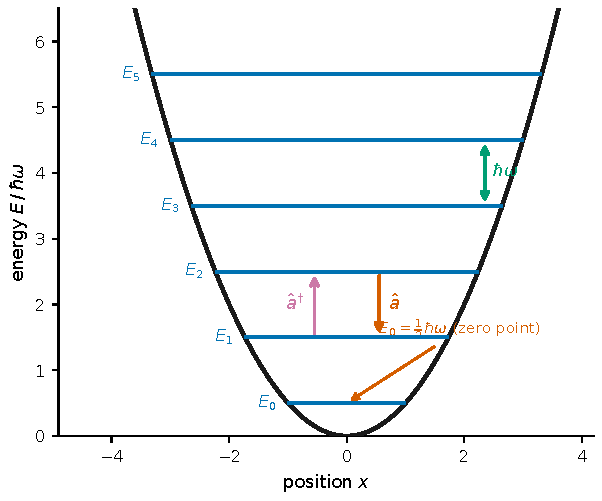
\includegraphics[width=0.6\linewidth]{figures/generated/edu_ch04/e04_energy_ladder.pdf}
\caption{The energy ladder of the quantum harmonic oscillator. In the potential well \(V(x)=\tfrac12 m\omega^2 x^2\), the allowed energies can only take the evenly spaced rungs \(E_n=\hbar\omega(n+\tfrac12)\): adjacent levels always differ by \(\hbar\omega\) (green double arrow), and the lowest level is not zero but the zero-point energy \(\tfrac12\hbar\omega\) (orange). The creation operator \(\hat a^\dagger\) lifts the system up one rung and the annihilation operator \(\hat a\) lowers it one rung. This ``constant one rung'' \(\hbar\omega\), for an electromagnetic field mode, is the energy of one photon.}
\label{fig:e04-energy-ladder}
\end{figure}

\section{A Preview: The Quantum State Closest to Classical Vibration}
\label{sec:e04-coherent}

The number state \(|n\rangle\) has the most definite energy, yet it is also the least ``like'' a classical vibration. Consider: the position of a classical oscillator traces a beautiful sinusoid over time, \(x(t)=x_0\cos\omega t\), but the position expectation of a number state \(\langle n|\hat x|n\rangle\) is identically zero, since by \eqref{eq:e04-xp-in-a}, \(\hat x\propto\hat a+\hat a^\dagger\) only turns \(|n\rangle\) into \(|n\pm1\rangle\), which is orthogonal to \(\langle n|\), giving inner product zero. That is, a quantum oscillator of definite energy has a position expectation that does not swing at all; in phase space it is a uniformly blurred ring, with no information whatsoever about ``which side it is on right now.'' This runs exactly counter to our everyday intuition about ``vibration.''

So which quantum state is the closest to classical back-and-forth swinging? The answer is the coherent state \(|\alpha\rangle\), defined as an eigenstate of the annihilation operator:
\begin{equation}
  \hat a\,|\alpha\rangle=\alpha\,|\alpha\rangle,\qquad \alpha\in\mathbb{C}.
  \label{eq:e04-coherent}
\end{equation}
\begin{formulaexplain}
The coherent state is an eigenstate of the annihilation operator \(\hat a\), with eigenvalue \(\alpha\) a complex number. The modulus of the complex number gives the mean photon number, its argument gives the vibration phase. It is the ``closest to classical'' quantum state.
\end{formulaexplain}
This definition looks strange at first: \(\hat a\) is not Hermitian, and its eigenvalue \(\alpha\) is allowed to be complex. But it is exactly this complex number that encodes amplitude and phase for us at once: \(|\alpha|\) sets how strong the vibration is (one can show the mean photon number \(\langle\hat n\rangle=|\alpha|^2\)), and \(\arg\alpha\) sets which phase it has swung to right now. One can show that the position expectation of a coherent state does indeed oscillate sinusoidally in time, and that it pushes the joint fluctuation of position and momentum down to the minimum allowed by the uncertainty relation; it is a small ``spot'' of light of constant size, translating uniformly around a circle in time, looking just like a classical point carrying a quantum blur.

Let us picture the two states on the same phase-space map (horizontal axis position \(x\), vertical axis momentum \(p\)). The image of the number state \(|n\rangle\) is a whole ring of uniform blur: its energy (the square of the radius) is definite, but the expectations of both position and momentum are identically zero and the phase is entirely undetermined, and you cannot say ``which point on the circle it has swung to right now,'' because it is smeared over the entire ring at once. The image of the coherent state \(|\alpha\rangle\), on the other hand, is a small, compact spot pinned to one point on the circle: it has a definite center, whose distance from the origin is about \(|\alpha|\) and whose azimuth is the phase \(\arg\alpha\), and this spot revolves uniformly around the circle in time, exactly reproducing the classical sinusoidal vibration \(x(t)\propto\cos\omega t\). Remember the difference of the two in one sentence: the number state is a ``ring smeared out into a full circle,'' the coherent state is a ``spot condensed to a point, translating around the circle.'' Figure~\ref{fig:e04-phase-space} draws these two phase-space pictures side by side.

\begin{figure}[tbp]
\centering
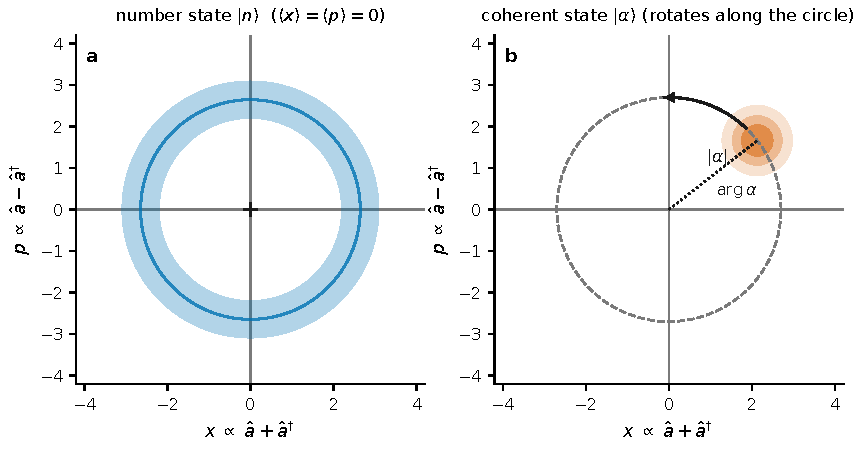
\includegraphics[width=0.92\linewidth]{figures/generated/edu_ch04/e04_phase_space_states.pdf}
\caption{Two extreme quantum states in phase space (horizontal axis \(x\propto\hat a+\hat a^\dagger\), vertical axis \(p\propto\hat a-\hat a^\dagger\)). Left: the number state \(|n\rangle\) has definite energy (the square of the ring radius is fixed) but spreads its probability uniformly over a full circle, with zero expectation of both position and momentum and completely undetermined phase, like a blurred ring. Right: the coherent state \(|\alpha\rangle\) condenses into a small, compact spot pinned to the circle of radius about \(|\alpha|\) and azimuth \(\arg\alpha\), revolving uniformly around the circle and reproducing the classical sinusoidal vibration.}
\label{fig:e04-phase-space}
\end{figure}

Here we merely set out the definition \eqref{eq:e04-coherent} and give an intuition; the detailed development (that its photon number follows a Poisson distribution, how it is written as a superposition of number states, why it is the natural starting point for lasers and stellar thermal light) is left to Chapter~\ref{chap:e06}. You need only remember one sentence: the number state is the extreme of ``most definite energy, most blurred phase,'' and the coherent state is the opposite extreme of ``clearest phase, most like classical swinging,'' and both use the same \(\hat a,\hat a^\dagger\).

\section{Chapter Summary}
\label{sec:e04-summary}

\begin{itemize}
  \item The entire quantum structure of the harmonic oscillator requires only one canonical commutation relation \([\hat x,\hat p]=i\hbar\). From it we define \(\hat a,\hat a^\dagger\) (Eq.~\eqref{eq:e04-adef}), and a term-by-term computation gives the core relation \([\hat a,\hat a^\dagger]=1\) (Eq.~\eqref{eq:e04-aacomm}); thereafter we can work entirely within the algebra of \(\hat a,\hat a^\dagger\).
  \item The Hamiltonian is rewritten as \(\hat H=\hbar\omega(\hat n+\tfrac12)\), where the number operator is \(\hat n=\hat a^\dagger\hat a\). That \(+\tfrac12\) is the zero-point energy \(\tfrac12\hbar\omega\), a direct consequence of the uncertainty relation forbidding the oscillator to be absolutely still.
  \item Using \([\hat n,\hat a]=-\hat a\) and \([\hat n,\hat a^\dagger]=+\hat a^\dagger\) we prove that \(\hat a,\hat a^\dagger\) lower/raise the eigenvalue rung by rung; using \(\langle n|\hat a^\dagger\hat a|n\rangle=n\ge0\) we force the eigenvalue to be a non-negative integer, with the ladder sealed at the floor by \(\hat a|0\rangle=0\).
  \item Normalization gives \(\hat a|n\rangle=\sqrt{n}\,|n-1\rangle\) and \(\hat a^\dagger|n\rangle=\sqrt{n+1}\,|n+1\rangle\), and the spectrum is an evenly spaced ladder \(E_n=\hbar\omega(n+\tfrac12)\). The adjacent-level spacing \(\hbar\omega\) is the energy of ``one photon.''
  \item The number state is the state of most definite energy and most blurred phase; the coherent state \(|\alpha\rangle\) (\(\hat a|\alpha\rangle=\alpha|\alpha\rangle\)) is the closest to classical vibration; see Chapter~\ref{chap:e06}.
\end{itemize}

\paragraph{Questions to Ponder.}
\begin{itemize}
  \item If you replaced \([\hat x,\hat p]=i\hbar\) by the classical \([\hat x,\hat p]=0\) and redid the derivation, what would \([\hat a,\hat a^\dagger]\) become? Would the energy levels still be discrete? This reveals to whom, exactly, the discrete levels are owed.
  \item The number state \(|n\rangle\) has position expectation \(\langle\hat x\rangle=0\), yet \(\langle\hat x^2\rangle\) grows with \(n\). Using \eqref{eq:e04-xp-in-a} and \eqref{eq:e04-ladder-action}, compute \(\langle n|\hat x^2|n\rangle\) and see whether it is proportional to \((n+\tfrac12)\), and explain the connection between this result and the zero-point energy.
  \item Why does ``absorbing one quantum of \(\hbar\omega\)'' mean ``one more photon'' for the electromagnetic field? Connect the energy ladder of the harmonic oscillator to the photon number and explain it in your own words.
\end{itemize}
